\section{Justering ift. matematisk model af PTS}
\label{ss:regulatorMat}
Som beskrevet i afsnit \ref{ss:ValgReg} er det valgt at implementere to PI-regulatorer.
Der tages udgangspunkt i den matematiske model af systemet, bestående af overføringsfunktionerne
\(G_{zoh,tilt}\) og \(G_{zoh,pan}\), som er diskretiseringer af de kontinuerte overføringsfunktioner.
Der skal findes to sæt koefficienter, \(K_P\) og \(K_I\), et sæt til hver regulator.
For at medtage den væsentligste ulinearitet, dødzonen, i regulatordesignet,
er det valgt at simulere systemet i Simulink.
I Simulink er den diskretiserede overføringsfunktion indsat sammen med en model for dødzonen,
målt eksperimentelt, samt PI-regulatoren. Det simulerede systems blokdiagram er illustreret i figur \ref{fig:simulink1}.
Da modellen indeholder ulineariteter er det valgt at starte med et simpelt gain \(K_P\) på 1,
og vha. "trial and error" prøve sig frem til koefficienterne.

\todo[inline, color=red!20]{Hvad menes der med dette?}

Begge regulatorer gives et parabelinput, og deres performance vurderes
efter deres evne til at følge parablen. Dvs. det er forsøgt at minimere trackingfejlen.

\begin{figure}[!th]
\centering
\begin{tikzpicture}[auto, node distance=2.6cm,>=latex']
%\begin{tikzpicture}[scale=0.9, every node/.style={scale=0.9}, node distance=2.6cm, =>latex']
\include*{./graphics/simulink1}
\end{tikzpicture}
\caption[Simuleret system]
		{Simuleret system. Tilbagekoblingsblokken angiver, at outputsignalet kvantiseres med et interval på \(q\mathrm{:} \frac{1}{1080}\),
		for at simulere motorens encoder feedback.
		\(D\left(z\right)\) er PI-regulatoren.}
\label{fig:simulink1}
\end{figure}
\todo[inline, color=red!20]{Vi skal snakke om figuren}


Med ovenstående metode blev koefficienterne i tabel \ref{tb:pidSimulink} fundet tilfredsstillende.
% Koefficienterne i tabel \ref{tb:pidSimulink} benævnes startkoefficienterne, da regulatorjusteringen
% ift. det fysiske system starter med disse værdier.
Trackingfejlen er afbildet i figur \ref{fig:pidSim1}, og som det ses af grafen, når den maks. 0,5\degree{} i simuleringen.

\begin{figure}[h!]
\centering
\begin{tabu}{l|[1.25pt]c|c|c}
      & \(K_P\) & \(K_I\) & \(K_D\)\\\tabucline[1.25pt]{-}
Tilt  & 240 & 85 & -\\\hline%0,248960\\\hline
Pan   & 240 &  100 & -
\end{tabu}
\captionsetup{type=table}
\caption[Regulatorkoefficienter]{Koefficienter fundet vha. simulering.}
\label{tb:pidSimulink} 
\end{figure}

\begin{figure}[h!]
\centering
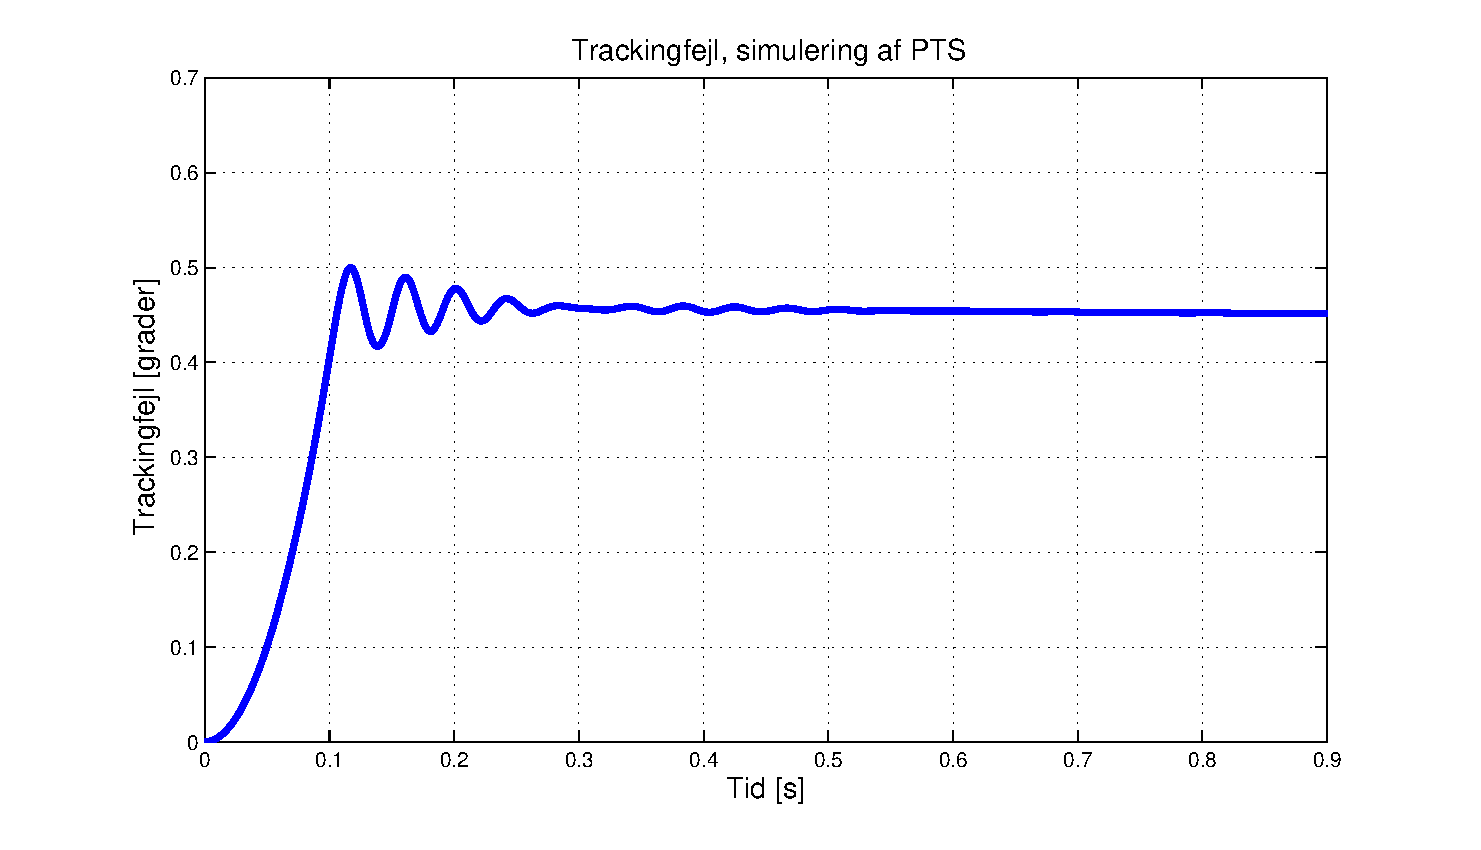
\includegraphics[width=0.7\textwidth]{./graphics/pidSim1.eps}
\captionsetup{width=0.6\textwidth}
\caption[Trackingfejl ved simulering]{Trackingfejl ved simulering af PTS med regulatorkoefficienterne fra tabel \ref{tb:pidSimulink}.} 
\label{fig:pidSim1}
\end{figure}
\todo[inline, color=red!20]{Denne test skal svare til en test vi laver på det rigtige system. Ellers er det ubrugeligt at se på en fejl og sammenligne den med en anden fejl i en anden situation}
De to regulatorer er med koefficienterne i tabel \ref{tb:pidSimulink} blevet afprøvet i praksis.
Figur \ref{fig:pidPhys1} viser pan og tilt-fejlsignalet i forhold til den kontinuerte lerdueparabel fra applikationen.

\begin{figure}[h!]
\centering
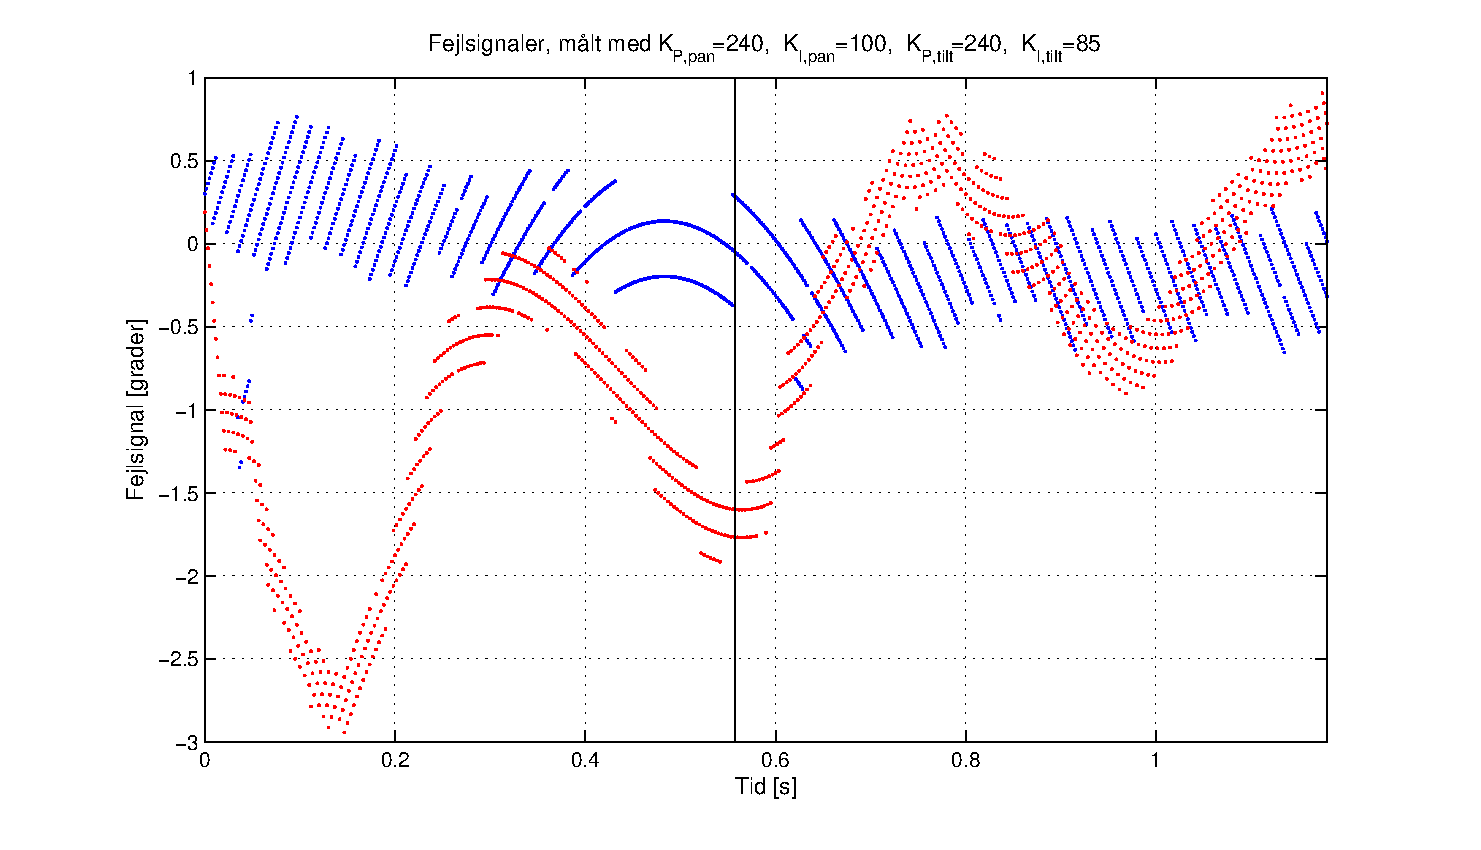
\includegraphics[width=0.7\textwidth]{./graphics/pidPhys1.eps}
\captionsetup{width=0.6\textwidth}
\caption[Fejlsignaler m. startkoefficienter]{Fejlsignaler m. startkoefficienterne fra tabel \ref{tb:pidSimulink}.
	De sorte lodrette streger angiver \(t_s=0,557 \text{ [s]}\).
	Pan-fejlsignalet er markeret med rødt, og tilt-fejlsignalet er markeret med blåt.
	Grafen indeholder målinger fra flere forsøg.} 
\label{fig:pidPhys1}
\end{figure}
\todo[inline, color=red!20]{En farve til tilt, en farve til pan. ingen kan se krydser eller prikker fra denne afstand.
Der er en enkel måling som ødelægger vores forsøg. Vi kan ikke vurdere at en tilt fejl på 0,9 er godt nok}


Som det ses på figur \ref{fig:pidPhys1} giver regulatoren til tilt et fejlsignal,
der maks. afviger 0,9\degree{} efter \(t_s\).
Pan-fejlen afviger derimod op til 1,8\degree{} efter \(t_s\).
Trackingfejlen er altså langt større end kravet på maksimalt 1,02\degree.
Det vurderes en yderligere manuel justering af koefficienterne på pan-regulatoren nødvendig.
Det vurderes på baggrund af det lave fejlsignal ved tilt at den fundne
PI-regulator for tilt er anvendelig i praksis.


\section{Manuel justering ift. fysisk PTS}
Ved at ændre på koefficienterne og analysere fejlgraferne justeres performance 
hen mod det ønskede.

På pan er der behov for en hurtigere og mere dæmpet reaktion,
og det vurderes derfor, at der på pan er brug for en PID-regulator.

\subsection{Valg af integratormætning}
Det vælges at sætte integratormætningen til 100 for begge regulatorer, da det vurderes, at der drages
fuld nytte af integratorleddet når \( K_I \cdot Integrator_{Max} > PWM_{Max} \).

\subsection{Tilføjelse af et D-filter}
Undervejs i den manuelle justering af PID-regulatoren til pan blev det fundet, at D-leddet ikke udnyttedes til fulde,
og at kravene ikke kunne overholdes med PID-regulatoren som den var.
Det valgtes derfor at tilføje et filter til D-leddet. 
Det betyder at D-leddet nu vægter tidligere ændringer i fejlsignalet. 
Filtret reducerer peaks i det differrentierede fejlsignal, der skyldes Zero Order Hold i upsamplingen (se afsnit \ref{subsec:upsampling}).

Der implementeres et 4. ordens FIR filter. Filtret er designet i MATLAB's grafiske fdatool og gør brug af at Kaiser vindue.
Filtrets step- og frekvensrespons kan ses på figur \ref{fig:d_filter_step} hhv. \ref{fig:d_filter_bode}. 

\begin{figure}[h!]
\centering
\subfloat[Steprespons for det implementerede filter.\label{fig:d_filter_step}]{%
	\hspace*{-0.6cm}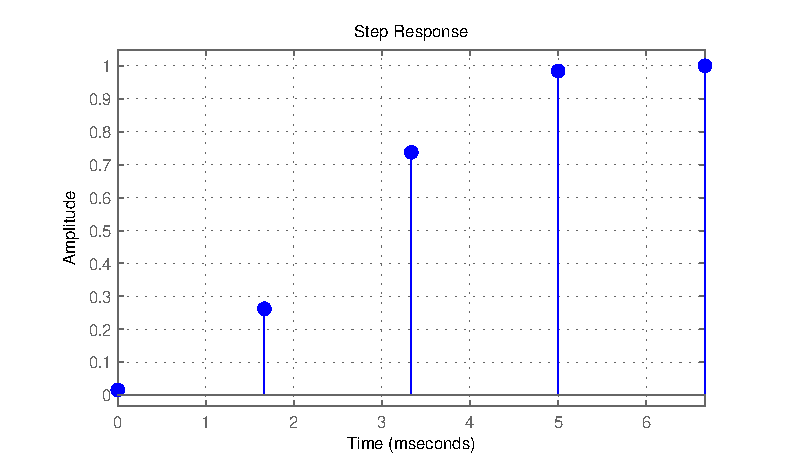
\includegraphics[width=0.57\textwidth]{./graphics/d-filter-step-small}
}
\subfloat[Frekvensrespons for det implementerede filter.\label{fig:d_filter_bode}]{%
	\hspace*{-1.15cm}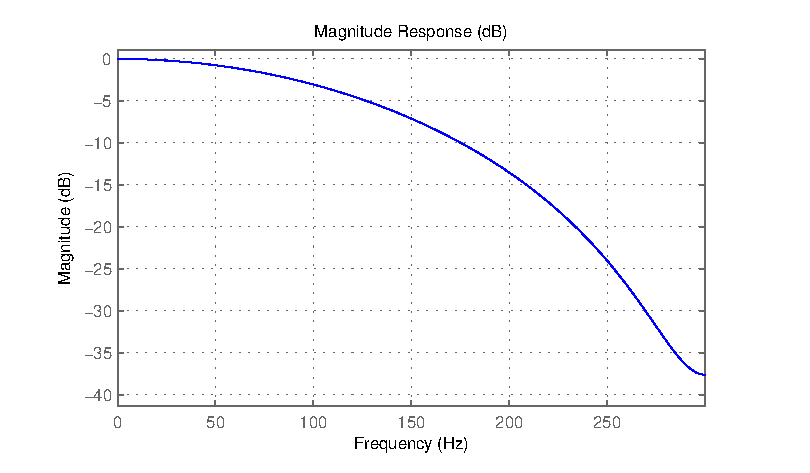
\includegraphics[width=0.57\textwidth]{./graphics/d-filter-bode-small}
	
}
\caption[D-filterets respons]{D-filterets step- og frekvensrepons.}
\label{fig:d_filter}
\end{figure}

\todo[inline, color=red!20]{større tidsakse så første og sidste spike kan ses}

\section{Endelig performance}
Efter adskillige test og finjustering af regulatoren, vurderes det at 
koefficienterne i tabel \ref{tb:PID_final} giver den bedst mulige performance 
for PTS. Denne performance ses i \ref{fig:PID_final}. Det ses at trackingfejlen 
holder sig inden for de 1,02$\degree$  pånær ved et par enkelte samples.

\begin{figure}[h!]
\centering
\begin{tabu}{l|[1.25pt]c|c|c}
      & \(K_P\) & \(K_I\) & \(K_D\)\\\tabucline[1.25pt]{-}
Tilt  & 240 & 85 & -\\\hline
Pan   & 100 & 110 & 3,8
\end{tabu}
\captionsetup{type=table}
\caption[Endelige regulatorkoefficienter]{De endelige regulatorkoefficienter.}
\label{tb:PID_final} 
\end{figure}

\begin{figure}[h!]
\centering
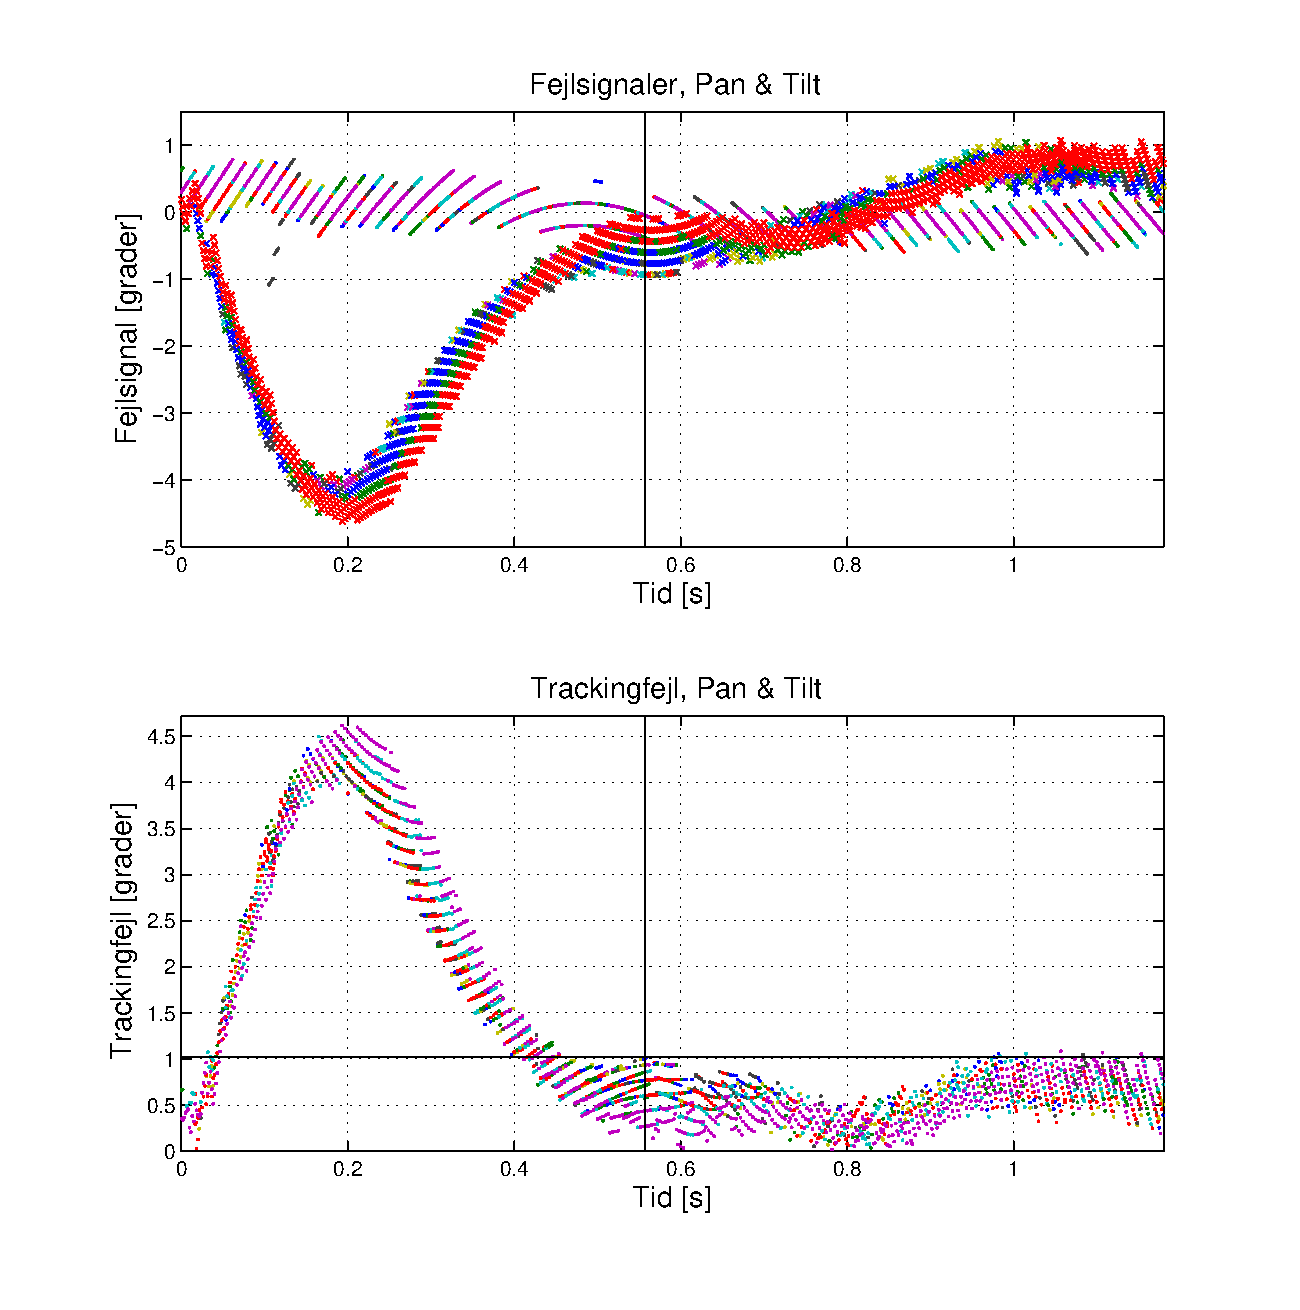
\includegraphics[width=1\textwidth]{./graphics/pidPhys2.eps}
\caption[Endelig performance]{Endelig performance. Fejlsignaler for Pan (rød) og Tilt (blå) øverst, trackingfejl nederst.
Testen er foretaget med koefficienterne fra tabel \ref{tb:PID_final}.
De sorte streger angiver kravene om Settling Time på under 0,557 [s] og trackingfejl på under 1,02\degree{}.
Grafen indeholder målinger fra flere forsøg.} 
\label{fig:PID_final}
\end{figure}

\todo[inline, color=red!20]{vi skal kigge på hvor meget vi er uden for og beskrive dette}

%
%\begin{figure}[h!]
%\centering
%\begin{tabu}{l|[1.25pt]c|c|c}
%      & \(K_P\) & \(K_I\) & \(K_D\)\\\tabucline[1.25pt]{-}
%Tilt  & 49 & 32,5 & 0\\\hline
%Pan   & 80 & 160 & 3,55
%\end{tabu}
%\captionsetup{type=table}
%\caption[Endelige regulatorkoefficienter]{De endelige regulatorkoefficienter.}
%\label{tb:PID_final} 
%\end{figure}
%
%\begin{figure}[h!]
%\centering
%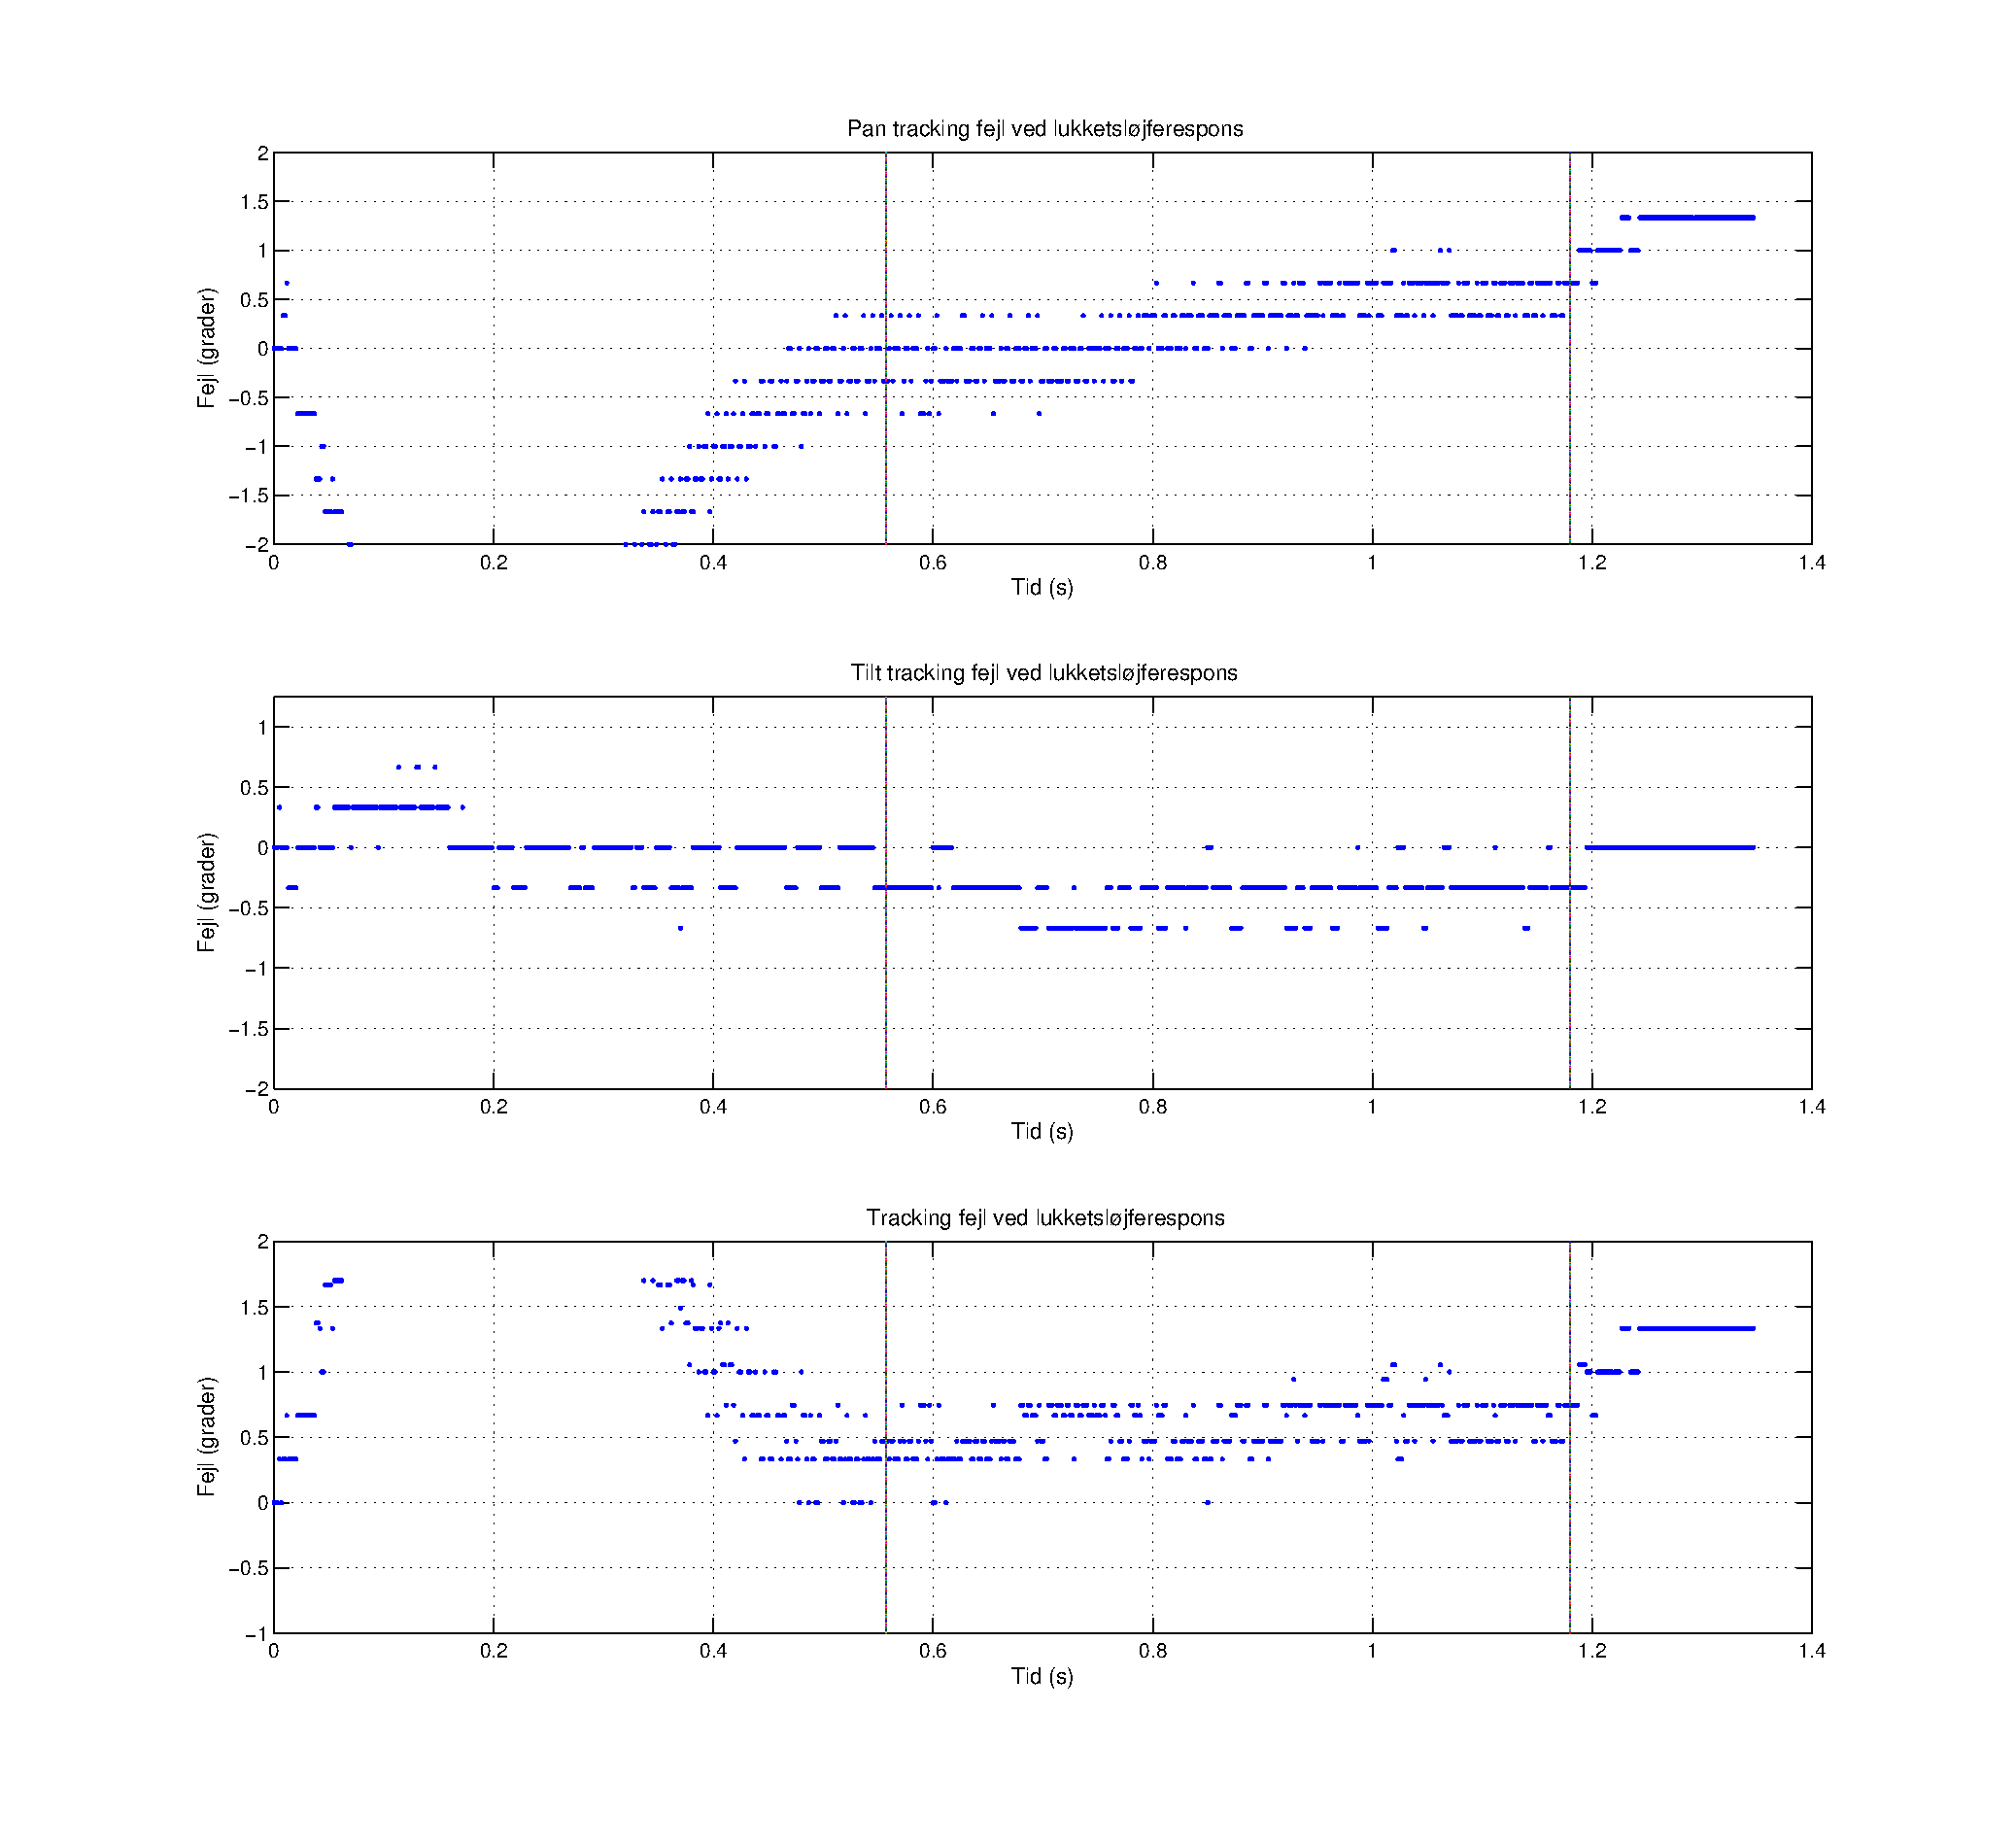
\includegraphics[width=1\textwidth]{./graphics/error_slut.eps}
%\caption[Endelig regulator koefficienter]{Trackingfejl målt i grader for hhv. pan og tilt samt den samlet trackingfejl. Testen tager udgangspunkt i koefficienterne fra  tabel \ref{tb:PID_final} og det ses at den samlet trackingfejl opfylder kravet til PTS.} 
%\label{fig:PID_final}
%\end{figure}

Det viste sig under justeringen at systemet er meget følsomt overfor slid i drivremmene mellem motorerne og Pan- og Tilt-rammerne.
Systemet kræver derfor kalibrering for at kunne fungere i praksis.

\section{Delkonlusion}
Ved "trial and error" blev regulatorkoefficienterne i Simulink justeret til at give den ønskede 
tracking performance ift. et parabelinput. Pan-koefficienterne giver dårlig performance i praksis.
Ved manuel justering blev et sæt PID-regulatorkoefficienter fundet til Pan, som gav bedre performance.
Det vurderedes nødvendigt at implementere et lavpasfilter til D-leddet.
Med det implementerede filter gav de justerede regulatorkoefficienter en performance,
der ikke ved alle forsøg levede op til kravspecifikationen. Ved nogle af forsøgene viste
systemet sig at leve op til kravene om en trackingfejl på under 1,02\degree efter 0,557 [s].
Systemet er følsomt overfor slid i drivremmene.